\documentclass{article}
\usepackage[utf8]{inputenc}

\usepackage{amsfonts}
\usepackage{enumitem}
\usepackage{amsmath}
\usepackage{xcolor}
\usepackage{hyperref}
\usepackage{graphicx}
\graphicspath{ {Figs/} }

\hypersetup{
    colorlinks=true,
    linkcolor=blue,
    filecolor=magenta,      
    urlcolor=cyan,
    pdftitle={Overleaf Example},
    pdfpagemode=FullScreen,
    }


\usepackage{geometry}
\geometry{margin=0.75in}



\begin{document}
\title{CMPSCI 389 Final Project Milestone 1 (HW5)}
\author{\textbf{Kamal Gurbanov, Graem Reeves}}
\date{Assigned: April 12 2024; Due: April 19 2024 @ 11:59 pm EST}

\maketitle

\begin{abstract}
    Now that we've had our fun coming up with ideas for our project we gotta do the lame part of actually working on it. These milestones are to help you not load up all of the work for the end of the semester -- don't worry too much about the quality of the writing, but y'know you still have to do all the work in them. \\ \\
    You should submit a pdf that you made using latex (sorry that's not gonna change), but your group only needs one submission and overleaf is great for that sort of thing. 
    
\end{abstract}

\section{Project description (25 points)}
In this section you have to finalize your choice of project and write a synopsis of it. You should include the following information (be specific):
\begin{enumerate}
    \item Motivation for your project (why this project? It's okay if you just think its fun/funny, but you should justify why you think its cool). Imagine you are trying to convince someone to care about your project.
    
    Our motivation for the final project is to create a song recommendation system. We're really excited about this project for a bunch of reasons! Firstly, digging into how recommendation algorithms work on platforms like Instagram, Spotify, and Netflix is just plain fascinating. Secondly, building our own recommendation system for music is a cool way to combine our love for tunes with some tech know-how. Plus, imagine having a model that can suggest songs we'll love—it's like having a personal DJ! And hey, the chance to show off our work in the Spotify 1,000,000 competition adds an extra kick of excitement and motivation.
    \item What type of model and training you are planning on using. 

    Our training type would probably be a unsupervised learning, and the model would be a Clustering model but we are still thinking about the model type, we might also use VAEs.
    
    \item The exact dataset that you will use to do this (it's really important to have a dataset and best to find them early)

    We will be using spotify 1.000.000 dataset, it has million songs and I already looked at the data, it has a lot of parameters which we can use as features in the latent space if we will be using VAEs. This dataset does not have a lot of null entries which is nice and the ones that were null, I cleaned them. Or we can create a score parameter taht will combine all the features and by that score parameter we would be able to cluster our datapoints.

    
\end{enumerate}

\section{Literature review (25 points)}
For this you need to find (and preferably read) some papers (or other resources -- but semantic scholar and paperswithcode.com will be super helpful) on projects as similar as possible to what you want to do. \\ \\
Then you should \textbf{include links} and short summaries of 3 that you think are the most related. 

\textbf{https://towardsdatascience.com/build-your-own-clustering-based-recommendation-engine-in-15-minutes-bdddd591d394}

This paper talks about creation of cluster based recomendation engine for the online courses, it explores more on the problem of what to do when there is no user interaction and also shows a step by step guide on how to create model using Kmeans clustering.

\textbf{https://journals.plos.org/plosone/article?id=10.1371/journal.pone.0278364}

This is the paper from 2022, it talks about other recommendation system implemented for Canadian online store, it first talks about classical ways of implementing recommendation systems and the most recent updates then it process to discussing what are the limitations of recommendation systems created by some other researchers. At the end it explains their own recommendation system created which uses clustering technique and supervised learning. I think this paper is discussing the subject pretty similar to our project.

\textbf{https://towardsdatascience.com/understanding-variational-autoencoders-vaes-f70510919f73}

This paper was written in 2019, it talks about the problems of classical autoencoder, and how variational autoencoder can solve those issues, by encoding input as a single point, VAE encodes it as a distribution over the latent space. It also talks about mathematical details of VAEs and at the end it introduces the counterpart for VAEs, and talks about  how GANs are more widespread than VAEs because how mathematically simple they are
\section{Preliminary / exploratory results (50 points)}

So far, we have experimented with using the Spotify 1,000,000 playlist dataset which contains the track lists of one million playlists with over two million tracks from three hundred thousand artists
In addition to the playlist and track names, the dataset also contains useful meta-data about the playlist like the like count and the playlist duration. \\ \\

In order to begin working on the dataset, most of the work that we have done so far has been related to data-handling and formatting. In the main.py file, we began by writing helper functions to seperate the
spliced data stored in json files, into pandas dataframes using the load\_df function. After, we then use process\_data function to convert each dataframe into a csv object that stores the processed data in order
to save computation. Within this function we also change the format of each row so that it is flat, by sorting each row by individual track instead of by playlist. This is because the playlist lengths vary and
the shape of the playlist format is difficult to work with. The old format transforms and reduces the data: \\
from the form: \{ PLAYLIST: \{NAME: XXX, TRACKLIST: [(multiple element list...)], more meta data, etc...\}\} \\to the form: \{ TRACK: \{NAME: XXX, ARTIST: XXX, ALBUM: XXX PLAYLIST: XXX\} \} \\
Additionally, this helps with cases where tracks exist in multiple playlists at the same time as it is easier to access that information \\ \\

After this, we use dictionaries to assign numerical values corresponding to each track name, artist name, album name, and playlist name in order to allow us to use a k-means algorithm on the data. We have experimented
using scikit learn in order to begin to try to cluster the tracks into groups. As far as how many clusters and what other relevant features we should use, will involve a lot of parameterization and testing to figure out.
You can see some of our initial results below. \\ \\

edit: i just realized we arent submitting the code to gradescope lol oops \\ \\ 

\begin{figure}[htb]
    \centering
    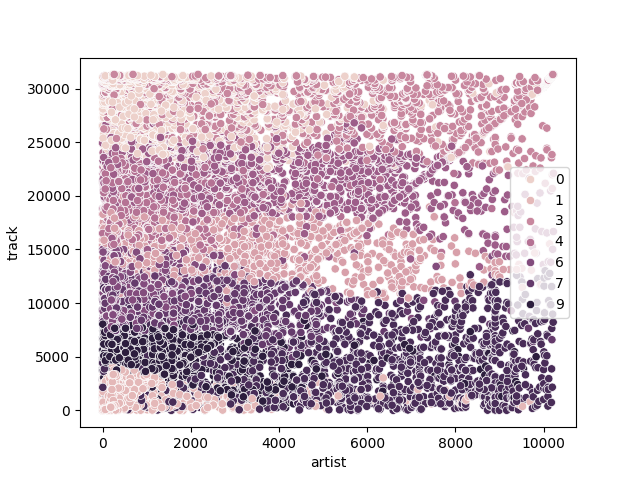
\includegraphics[width=0.8\textwidth]{Figs/cluster-artist:track.png}
    \caption{ Clustering visualized through artist and track name of tracks from 1000 playlists}
    \label{fig:net}
\end{figure}
\begin{figure}[htb]
    \centering
    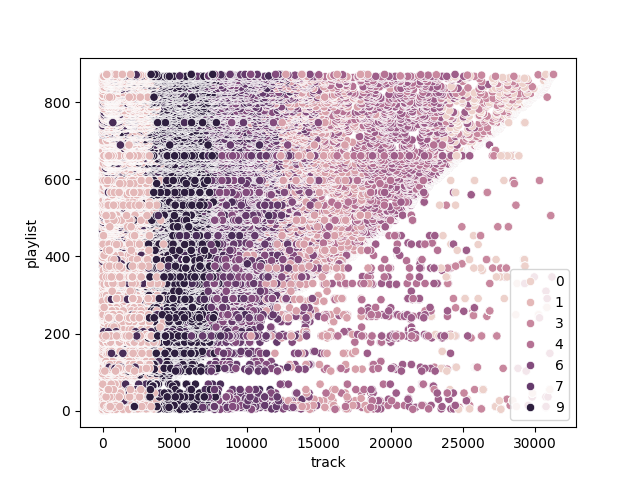
\includegraphics[width=0.8\textwidth]{Figs/cluster-track.png}
    \caption{ Clustering visualized through track and playlist names from 1000 playlists}
    \label{fig:net}
\end{figure}

\end{document}